\documentclass[12pt]{article} % For LaTeX2e
%\documentstyle[nips14submit_09,times,art10]{article} % For LaTeX 
%\usepackage{nips15submit_e,times}
 \usepackage{times}
%\usepackage{hyperref}
%\usepackage{url}
% \usepackage[margin=1in]{geometry}

\linespread{1.5}
\usepackage{amsmath,amsthm,amssymb}
\usepackage{subcaption,graphicx}
\usepackage{tabularx}
\usepackage{float}
\usepackage{tabularx}
\newcommand{\N}{\mathbb{N}}
\newcommand{\Z}{\mathbb{Z}}
\usepackage[round]{natbib}
\usepackage[margin=1.25in]{geometry}
% 2.09

\title{Sentence Encoders for Semantic Textual Similarity - A Survey}

% The \author macro works with any number of authors. There are two commands
% used to separate the names and addresses of multiple authors: \And and \AND.
%
% Using \And between authors leaves it to \LaTeX{} to determine where to break
% the lines. Using \AND forces a linebreak at that point. So, if \LaTeX{}
% puts 3 of 4 authors names on the first line, and the last on the second
% line, try using \AND instead of \And before the third author name.

\newcommand{\fix}{\marginpar{FIX}}
\newcommand{\new}{\marginpar{NEW}}

%\nipsfinalcopy % Uncomment for camera-ready version

\begin{document}


\maketitle


\begin{abstract}
Semantic similarity between two sentences is a basic language understanding problem that is applicable in many natural language processing applications. We replicated and extended existing works proposed in Association of Computer Linguistics' SemEval competitions to evaluate semantic models. We gathered features such as the length, vector spaces and text difference and implemented three models: SVM, RF, and CNN to measure semantic textual similarity. 
\end{abstract}

\section{Background}
\subsection{Semantic Textual Similarity (STS)}

Semantic Textual Similarity (STS) is a task of finding how closely two sentences are related in terms of meaning \cite{cer2017semeval}. Semantic similarity between two sentences is a basic natural language understanding problem that is applicable in many natural language processing applications such as web search, information retrieval, evaluation of machine translation system and automatic text summarization, etc,. Any natural language understanding problem starts with the challenge of describing words and sentences to machine understandable representation i.e a vectorial representations that encodes its whole meaning. These representations are also called distributional representations and the area of research on this problem is called Distributional Semantics. The model that learns these representation are called encoders. Since 1990, many vector space models have been proposed to estimate continuous representations of words  such as Latent Dirichlet Allocation (LDA), Latent Semantic Analysis (LSA). \cite{bengio2003neural} learnt the word representations while training neural language model. Later in 2008, the effective use of pre-trained word vectors in various task were explained by \cite{collobert2008unified}. \cite{mikolov2014word2vec} proposed a shallow neural network model for learning word representation which performed very well in capturing the general syntactical and semantic information. Recenlty, researchers have focused more in learning a general sentence representations that would capture its proper semantics. 

 To stream line the research and standardize the dataset related to semantic analysis task, Association of computer linguistics started organising shared task since 2012. For decade, traditional machine learning algorithms such as support vector machine or logistic regression were to used to solve the any NLP tasks.  

For training and test of the STS model, we used data published in SemEval 2012-SemEval 2017 which includes the collection of STS dataset created using corpus from various domains like News headlines from the RSS feed of the European Media Monitor, Image captions from Flickr, Pairs of answers collected from Stack Exchange, student answers paired with correct reference answers from the BEETLE corpus, and Forum discussions about beliefs from the DEFT Committed Belief Annotation dataset \cite{sem-eval2105}. The performance of the model is measured using Pearson correlation of the predicted score with the human judgment score given in the dataset.



\subsection{Research Contributions}
\subsection{Contributions}


\section{Related Work}

Despite of developing a number of learning algorithms for representing words and sentences, generating high quality and efficient sentence representations remains an unsolved problem until the present \citep{conneau2017supervised}. A efficient sentence representation that consist of the whole meaning with context is important as it can be used across various tasks with minimal adaption. This property results in smooth transfer of the learning to the model that learns any specific task. These sentence representations are used in many NLP task likes Semantic Textual Similarity, Paraphrase Detection, Sentiment Analysis, Sentence classification, as few are mentioned in here. The tasks are generalisation of various applications  These  I focus on STS task as \cite{conneau2017supervised} has proposed the natural language inference task appears to capture This work proposes a comparison study on different encoder models used for STS tasks and their importance in generating a  

Since 2012, SEM-EVAL shared task for semantic textual similarity has been held by Association of Computer Linguistics to vitalize its research area. In 2012, supervised models based on the lexical and syntactic features of the sentence pair showed promising results on measuring semantic relatedness. These systems gave 52\% - 59\% correlation on various datasets by using regression models consisting of various similarity measure as its input features. Later, the unsupervised models did well for next two year in row using the WordNet knowledge and the LSA similarity measures which assume that the words with closer meaning highly co-occur in the text corpora. \cite{han2013umbc_ebiquity} proposed three approaches that involved LSA similarity model, semantic similarity model based on the alignments quality of the sentences and support vector regression model that had features from different combination of similarity measures and the measures from other two core models. It is observed that using n-gram overlap feature increased LSA similarity model. Out of three models proposed by \cite{han2013umbc_ebiquity}, alignment based system gave 59\%- 74.6\% pearson correlation on four different dataset. Using this model's alignment quality as one of the feature in the Support Vector Regression model improved the correlation score to 78 \%.  Various supervised models using unigram/bigram overlap, vector distance, and cosine similarity of sentence embedding were proposed \citep{agirre2015semeval}.
 
 \cite{tian2017ecnu} proposed a system that adapted ensemble learning techiques to solve the Tectual Entailment and STS task using same set of features. The combination of classical NLP models like Support Vector Machine , Random Forest , Gradient Boost and a deep learning model are used in this system. For classical NLP models,single sentence and sentence pairs feature sets are hand engineered based on the properties like N-gram overlap, syntax, alignments, word sequence, word dependency, word representations, etc. In SEM-EVAL 2017, this mixed ensemble model gave 81 \% pearson correlation outperforming all the neural models presented in that shared-task event.

Although using hand-crafted features with above mentioned models perform well, it has some drawbacks like tuning the features extracted on addressing the corpus from new domains, etc. Recent approaches in deep learning continues to prove the problem of semantic text matching can be  handled in a efficient way \cite{cer2017semeval}. The problem of distributional word match can be generalized to the problem of the distributional sentence match by using deep learning approaches. This helps in effectively learning the individual meanings from embedding of all the words in the sentence and derives a meaningful sentence representation from the word vectors. This section discusses about the  top ranking models presented in SEM-EVAL 2017 that has been proposed to build sentence representations and predict sentence relatedness. 

\subsection{CNN Architecture} 
\cite{shao2017hcti} presented a simple Convolutional neural network model for Semantic Textual Similarity task. This model constsis of CNN model and fully connected neural network (FCNN). CNN takes pre-trained word vectors from Glove \cite{pennington2014glove} enhanced with handcrafted features as its input. It enhances word vector to task specific form in the convolutional layer and max-pooling generates the task-dependent sentence representation. FCNN generates the similarity score ranging from 0-5. This model ranked 3rd in SemEval-2017 with 78 \% correlation on STS task. 

\subsection{Skip-ThoughtVector}
 \cite{kiros2015skip} proposed Skip-Thought model based on skip-gram objective from Word2Vec \cite{mikolov2014word2vec}. For any three consecutive sentence in the document $S_{i-1}, S_{i}, S_{i+1}$, the Skip-Thought model predicts the previous sentence $S_{i-1}$ and next sentence $S_{i+1}$ given any sentence $S_{i}$.
This work focus on training a encoder-decoder model. A varient of recurrent networks consisting of gated recurrent units (GRU) \cite{cho2014learning} is used as a encoder to map input sentence into a generic sentence representations. RNN with conditioned GRU used as language model to decode the sentence representation and predict surrounding sentence $S_{i-1}$ and $S_{i+1}$. On evaluating on semantic relatedness task, Skip-Thought outperformed all systems proposed in shared task SemEval 2014 \cite{marelli2014semeval} and was outperformed by dependency Tree-LSTM model.


\subsection{LSTM Networks} 

\cite{tai2015improved} proposed a recurrent neural networks(RNN) with tree based LSTM units. Child-Sum Tree-LSTM and N-ary Tree LSTM are two variants. Given a sentence synatctic structure in form dependency tree of the words, Tree-LSTM networks are capable of integrating the child node's information. The Tree-LSTM units in each node t consist of input gate $i_{t}$, output gate $o_{t}$, a cell unit $c_{t}$ and a hidden output $h_{t}$. Unlike Standard LSTM, the parent node has one forget gate $f_{tk}$ for each child node \textit{k} in the Tree-LSTM. This property allows selective usage of child information. Previously proposed RNN models with sequential LSTM units have limited ability to capture meaning difference in the two sentence raised due to word order and synactical structures. Tree-LSTM address its issue by computing its hidden layer output as function of the outputs from its children hidden units and input vector. 

On modelling semantic relatedness, the input $x_{t}$ denotes the word vectors of sentence parse tree. The proposed model retains the information of more distant word from the current word compared to other exisiting models. These properties makes the model effective in highlighting the semantic heads in the sentence. It also captures the relatedness of two phrase which has no word overlap. With these propoerties, Tree LSTM performs better than existing sequential RNN-LSTM models and models with hand engineered features on predicting the semantic relatedness of two sentence.But one of the major downside is dependency tree-LSTM relies on parsers for dependecy tree input which computationally expensive to collect and does not exist for all languages making it inefficient in cross-lingual sentence representations.

\subsection{Sent2Vec}
\cite{pagliardini2017unsupervised} proposed a simple unsupervised objective Sent2Vec to train a generic distributed representations for sentences.The main contribution of Sent2Vec is its low computational cost for both training and inference relative to other existing state-of-art model. This model is a extension of CBOW training objective from Word2Vec\cite{mikolov2014word2vec} to sentence context.

\subsection{InferSent}
\cite{conneau2017supervised} investigated on performance of various supervised encoders in learning universal sentence representations. They hypothesized that textual entailment task is good choice for learning the universal representations and demonstrated the hypothesize with various enoder models. To prove that sentence representations learnt are universal, the representations learnt from unsupervised and proposed hypothesis was used in 12 different transfer task namely Caption-Image retrievel, Paraphrase detection, Entailment/semantic relatedness, sentiment analysis, etc,. As the result of their experiments, Bi-LSTM with max-pooling trained on Natural Langugae Inference Task(Textual Entailment) using standford generated best sentence representations outperforming SkipThought \cite{kiros2015skip} and FastSent \cite{hill2016learning}.
 

\section{Proposed Work}

A wide variety of supervised and unsupervised encoders  for learning sentence representation are proposed by NLP researchers in recent times. However, there is a lack of knowledge about the encoding techniques that can capture useful, generic semantic information \citep{conneau2017supervised}. Supervised neural models captures the bias in the dataset effectively. This feature is a downside because it learns the task very well and forgets to capture general useful information over time leading to poor generalization. On the contrary, unsupervised learning models gives more importance to general information, therefore, failing to specialize the model for any specific task. Many reasons impact how the basic semantics of a sentence is being captured while learning. An important reason to note is the task for which the model is trained. Similarly, the encoder's architecture for both supervised and unsupervised neural models also impacts the learning in different ways. A comparison study on these encoder's architecture will enable us to gain better insight on how better sentence representations are captured.

%To infer more insights on the techinques that yield state of the art performance on capturing the semantics of the sentence, we compare few models presented in SemEval-2017 \cite{cer2017semeval} that showed promising results on STS shared task.

In this project, I propose to perform  a systematic comparsion of different encoder techniques for generating sentence representations and their abiltiy to capture semantics of the sentence. To do this, I am implementing and studying the following models: support vector machine (SVM), Random Forest (RF), Convolutional Neural Network Enoder \cite{shao2017hcti} and BiLSTM RNN with max-pooling \citep{conneau2017supervised}. These models will be implemented using sci-kit learn, PyTorch and Keras library. As demonstrated in \cite{conneau2017supervised}, Recognizing Textual Entailment (RTE) captures natural language inference, we will train our  encoders on standford Natural Language Inference (SNLI) corpus  \cite{bowman2015large} and SICK (Sentences Involving Compositional
Knowledge) dataset \cite{marelli2014semeval} for semantic relatedness and RTE tasks.

The main objective of this comparison study is to understand the quality of the sentence representations and to answer the following questions:

\begin{itemize}
	\item What are the vital features in prediction while using machine learning models ?
	\item Effectiveness of the traditional machine leanrning models ?
	\item What are the trade-offs that neural networks
	incur as opposed to the traditional machine leanrning models?
	\item What is the preferable neural network architecture for learning better sentence representations? 
	\item Since the dimensionality is directly effect on the memory requirements and processing time, Which encoder ensures to learn good representations with what dimensionality size have good trade-off between accuracy and training time. 
	\item What is the impact of various activations functions used in the enoders hidden layers?
\end{itemize} 

%Both the RNN models investigated with mean and max pooling over the hidden representations separately. 



 
	 
	 
	 
	 
%	 , far less is known about  across many task. for representing the sentence that captures semantics and syntactic  focusing on the semantic relatedness and diferent appro

\section{Implementations}
%	\subsection{Feature Engineering}
	In this section, we will discuss the models that we are exploring. We implemented the models proposed in \cite{shao2017hcti} and further extended them and measured their performance using Pearson's Correlation.
	
	\subsection{A Simple CNN Model For STS Task}
		This section explains the deep learning model used for semantic sentence similarity. The two main components of this model are convolution neural networks(CNN) based sentence representation model and fully connected neural networks(FCNN) used as the multi-class classifier. The CNN architecture consists of two convolution networks that work in parallel to mapping the two sentences to a vector space. The distributional vectors of the sentence pairs are used by FCNN to classify its sentence similarity score. In the following, we first describe our sentence model for mapping sentence pair to their intermediate representations and then explain how these representations are used to classify the relatedness score.
	
	\subsubsection*{Sentence Model using CNN}
	Our CNN architecture for mapping sentences to feature
	vectors inspired from \cite{shao2017hcti} is shown on Figure 1 . This architecture consists of two 1-dimensional convolution layer and a max pooling layer. The objective of this network is to convert the raw sentence into vector representations from \cite{glove}, pre-trained 300 dimension word embeddings of all the words \{$w_{1}, w_{2},...,w_{|s|}$\} present in the sentence.
	
	The input sentence to the convolution layers is treated as a sequence of real valued number where the real valued integers are retired from the integer-word mapping present in the vocabulary V. The vector representaion of all the word $ w \in \mathbb{R}^{d}  $ drawn from embedding matrix  $ W \in \mathbb{R}^{d \times |V|} $ in the embedding layer. To enhance the word representation with respect to this task, a true flag for word overlap is added as a additional dimension into the word vector representation for each word in the sentence. Then the CNN network applies convolution and max pooling operation to find the optimal feature vectos for the sentence that capture its semantics. 
	
	The idea behind the convolution layer is to learn the features which identifies the relationship between n-gram of the sentence using weight vectors \textit{m} $\in \mathbb{R}^{|m|}$ . The $1 \times 1$ weight vector \textit{m} also known as filters of the convolution is used. This convolution operation is followed by applying Relu activation function to learn non-linear decision boundaries. This filters out the insignificant features learnt in previous operation. The output from convolution layer is passed to max pooling layer with pool size (1, $|S|$) where the semantic information learnt is aggregated and reduuces representation dimension from $1 \times |S| \times 300$(word vec dimension) to $1 \times 300$(word vec dimension).The convolution layers along with Relu activation function and max pooling acts as non linear  feature detector for the given sentence. The output sentence representation from CNN is used to find Semantic Difference Matrix by performing a series of operation on the two sentence vector. 
	
	\begin{figure}[!tbp]
		\centering
		\begin{minipage}[b]{0.43\textwidth}
		\centering
		\label{CNN_1}
		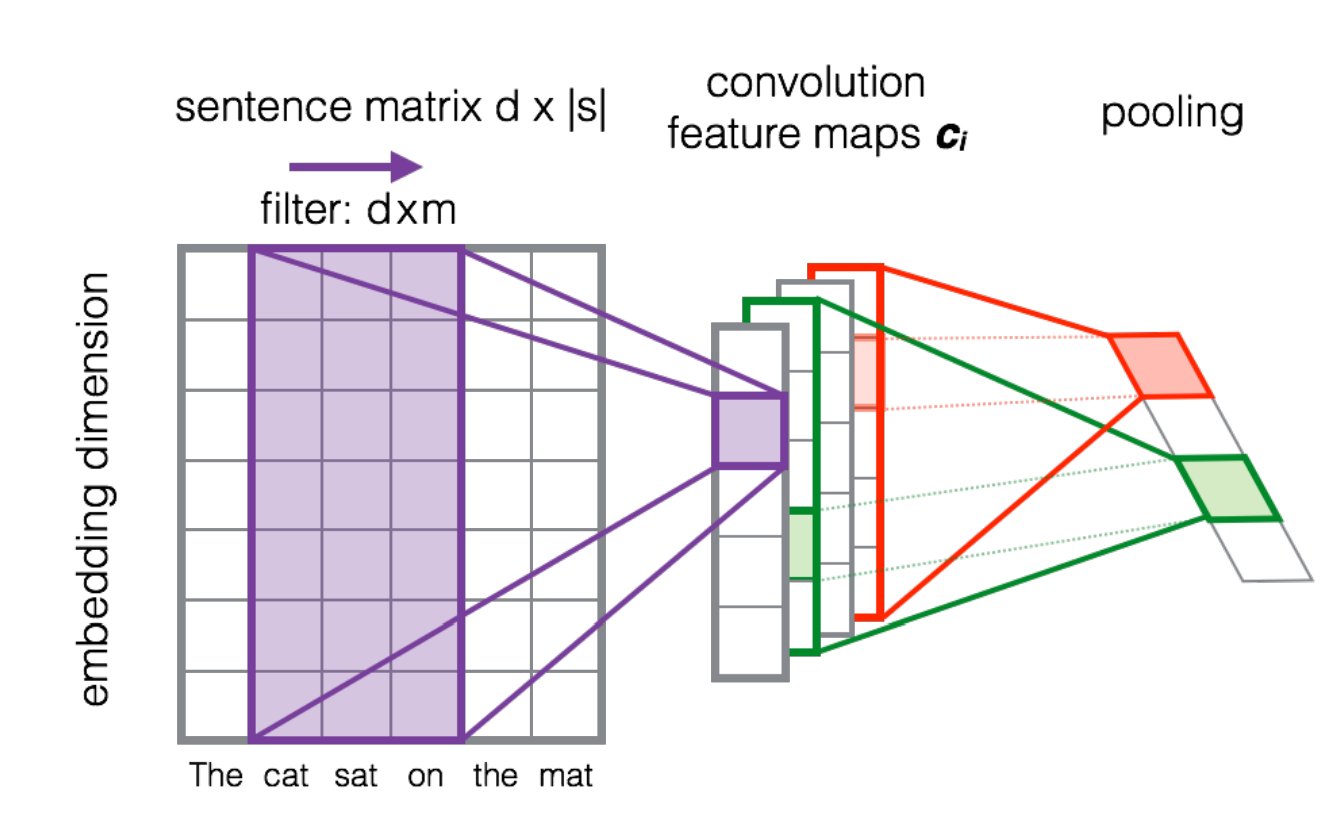
\includegraphics[scale=0.20]{CNN_sentModel.png}
		\caption{CNN Sentence Model \cite{severyn2015learning}}
		\end{minipage}
		\hfill
		\begin{minipage}[b]{0.3\textwidth}
		\centering
		\label{params}
		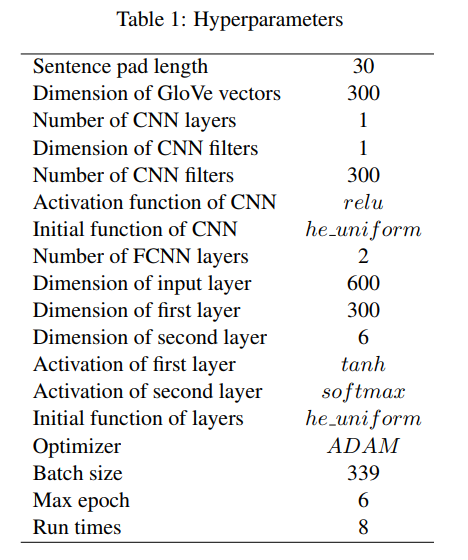
\includegraphics[scale=0.35]{hyperparameters.png}
		\caption{Hyperparameters for FCNN \cite{shao2017hcti}}
		\end{minipage}
	\end{figure}
	
	
	\subsubsection*{Semantic Difference Matrix}
	The semantic difference matrix is generated by concatenating the vector difference and vector product of two sentence representation. This  matrix is used to classify the similarity measure using fully connected neural network(FCNN) with 2 dense layers. 
	
		\begin{align*} 
			SDV & =(|SV_{1}- SV_{2}|.(SV_{1} \circ SV_{2})) \\
		\end{align*}
	
	\subsubsection*{Similarity Measure using FCNN}
	
	 This network consists of one hidden layer of size 300 nodes and a output layer of size 6.The hidden layer applies \textit{tanh} activation function and the output layer applies softmax layer. The softmax layer calculates the probability over the six score labels. The hyper parameters of this network is shown Figure \ref{params}
	 
	 Finally, the model is trained using the categorical cross-entropy loss: given a vector of probabilities p for a training pair of sentences, if the correct similarity category corresponds to index i of p, the model will evaluate the loss as $L = − log(pi)$.
	 

	\section{Expected Results}
	
	\section{Evaluation}
    
    
	\section{Conclusion}
   
\bibliographystyle{plainnat}
\bibliography{sample}   

\end{document}